\section{\uppercase{Vorgehen}}

\subsection{App-Entwicklung}

\noindent Parallel zu diesem Projekt befindet sich auch der Server, der verwendet werden soll in der Entwicklung. Zum Testen des Servers wurde eine Web\-ober\-fl\"ache bereitgestellt.\footnote{http://34.238.158.85/MDSD-2017\_2018/doc/swagger-ui-master/dist/index.html} \\
Um die Umsetzung eines Zugriffs auf einen REST-Service in Android zu testen, wurde ein Prototyp auf klassische Weise programmiert. Das bedeutet, dass der Code in Android Studio ausgehend von einem leeren Projekt entwickelt wird. Dabei werden einerseits Erkenntnisse generiert, wie die Verbindung mit dem REST-Server funktioniert und allgemein, wie die App in Android umgesetzt wird, sodass man sieht, was in welche Dateien geschrieben werden muss und wie diese strukturiert sind.\\
Au\ss{}erdem wurde die App auch mit Hilfe von $\text{MD}^2$ umgesetzt. Dabei sieht man die Grenzen die bei $\text{MD}^2$ noch bestehen. Den Code der von $\text{MD}^2$ generiert wurde kann man dann analysieren und mit dem auf klassische Weise erzeugten Code vergleichen. Da bei der Erzeugung des $\text{MD}^2$-Codes ebenfalls Muster entstehen, die im Rahmen der in Android g\"ultigen Strukturen bestehen, kann man diese nutzen, um ein weiteres Programm zu erzeugen, dass die fehlenden Elemente automatisch erzeugt.\\
Die Abbildung \ref{fig:Arbeitsschritte} zeigt das Vorgehen bei der Entwicklung der $\text{MD}^2$-App.

\begin{figure}[!h]
	%\vspace{-0.2cm}
	\centering
	{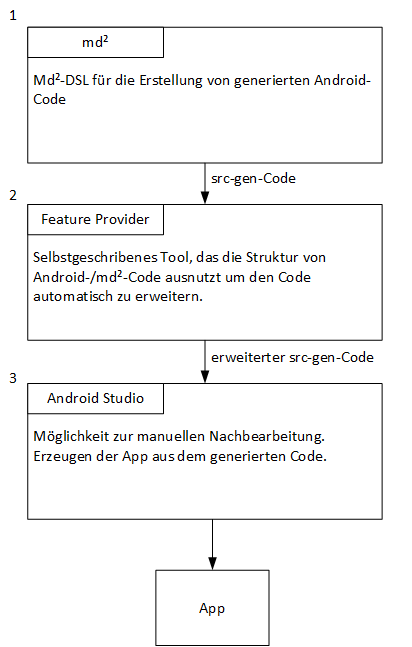
\epsfig{file = Abbildungen/Arbeitsschritte.png, width = 5.5cm}}
	\caption{Es werden die einzelnen Arbeitsschritte dargestellt. Die Zahlen geben die Reihenfolge der Schritte an. An den Pfeilen steht die Ausgabe des Vorg\"angerschritts, die als Eingabe des n\"achsten Schritts dient.}
	\label{fig:Arbeitsschritte}
\end{figure}

\noindent Der Code, der von $\text{MD}^2$ erzeugt wird, wird in einen Ordner mit dem Namen "src-gen" gespeichert. Auf diesem Code arbeitet der Feature Provider weiter. Das Ergebnis des Feature Providers wird in dem gleichen Ordner gespeichert. Nachdem der Code erweitert wurde kann er mit Android Studio ge\"offnet werden. Bei Bedarf k\"onnen manuelle Ver\"anderungen an dem Code vorgenommen werden. In Android Studio kann die App dann kompiliert und getestet werden.

\subsection{Feature Provider-Entwicklung}
Bei der Entwicklung des Feature Providers werden die Erkenntnisse der klassischen Programmierung ausgenutzt. Dabei werden allgemein g\"ultige Konzepte benutzt, sowie das Wechseln einer Activity mit Hilfe eines Intents. F\"ur die Umsetzung der Kommunikation mit einem REST-Service gibt es verschiedene Bibliotheken. Der Feature Provider benutzt ausschlie\ss{}lich die Bibliotheken, die bei der klassisch programmierten App benutzt wurden.\\
Zuerst wurde die Benutzeroberfl\"ache entwicklet, die es erm\"oglicht die entsprechenden Einstellungen auszuw\"ahlen. Besonders wichtig ist, die Auswahl des "src-gen"-Ordners, da der Absolute Pfad zu diesem Ordner auf jedem Ger\"at anders ist.\\
Danach wurde die Funktionalit\"at des Erzeugens der Features implementiert.\\
Zur Entwicklung der Funktionalit\"at des Feature Providers wurde in den von $\text{MD}^2$ erzeugten Code geschaut an welcher Stelle zus\"atzlicher Code eingef\"ugt werden muss, oder wo der Code durch anderen ersetzt werden muss. In der klassischen App wurde der Code gepr\"uft, wie die Funktionalit\"at umgesetzt wurde. Bei der Erstellung des Feature Providers wurden dann einige Klassen direkt \"ubernommen mit einigen Ver\"anderungen. Nach der Erzeugung einer neuen Funktion des Feature Providers wurden die in Abbildung \ref{fig:Arbeitsschritte} dargestellten Arbeitsschritte durchgef\"uhrt um zu testen, ob die App dann noch funktioniert und um zu sehen, dass das gewollte Feature hinzugef\"ugt wurde.